\documentclass[11pt]{article}
\usepackage{fullpage}
\usepackage[page,toc,title]{appendix}
\usepackage{verbatim}
\usepackage{moreverb}
\usepackage{amsmath}
\let\verbatiminput=\verbatimtabinput
\def\verbatimtabsize{4\relax}
\usepackage{tikz}
\usetikzlibrary{arrows,automata, positioning}
\usepackage{array}
\usepackage{booktabs}
\usepackage{minted}
\usepackage{parskip}
\usepackage{float}
\usepackage{pbox}
\usepackage{makecell}
\usepackage{adjustbox}
\usepackage{color}
\definecolor{rltred}{rgb}{0.75,0,0}
\definecolor{rltgreen}{rgb}{0,0.5,0}
\definecolor{rltblue}{rgb}{0,0,0.75}
\definecolor{berkeleyblue}{rgb}{0.19,0.35,0.52}

\usepackage[%pdftex,
    colorlinks=true,
    urlcolor=rltblue,               % \href{...}{...}
    anchorcolor=rltbrightblue,
    filecolor=rltgreen,             % \href*{...}
    linkcolor=rltred,               % \ref{...} and \pageref{...}
    menucolor=webdarkblue,
    citecolor=webbrightgreen,
    pagebackref,
    pdfpagemode=UseNone,
    bookmarksopen=true]{hyperref}
\usepackage{graphicx}
\usepackage{hyperref}

\newcommand{\instbit}[1]{\mbox{\scriptsize #1}}
\newcommand{\instbitrange}[2]{~\instbit{#1} \hfill \instbit{#2}~}

\newcommand{\currentSemester}{Spring 2023}
\newcommand{\projectSpecVersion}{2.21}

\newcommand{\blockDiagramTaskName}{Checkpoint 1}
\newcommand{\blockDiagramDueDate}{April 3}

\newcommand{\baseCPUTaskName}{Checkpoint 2}
\newcommand{\baseCPUDueDate}{April 10}

\newcommand{\finalCheckoffDueDate}{May 4}

\newcommand{\finalReportDueDate}{May 8}

\newcommand{\semesterName}{sp23}

%Also, change the info in minted blocks.  This includes the "Setting up your Code Repository" section and the "Setting up the Vivado Project" section




\begin{document}

\hypersetup{pageanchor=false}
\thispagestyle{empty}

\begin{center}

\includegraphics[width=0.25\textwidth]{figs/Seal_of_University_of_California_Berkeley.png}
\end{center}
\begin{center}
\LARGE{
\color{gray}
\bf EECS151/251A \\
\currentSemester \\
Final Project Specification \\
}
\end{center}

\vfill

\begin{center}
\Huge{
\color{berkeleyblue}
\bf RISCV151 \\
}
\end{center}

\vfill

\begin{center}
\LARGE{
\color{gray}
Version \projectSpecVersion \\
}
\end{center}

\vspace{3mm}

\begin{center}
\large{
TA: Rahul Kumar, Yukio Miyasaka, Dhruv Vaish
}
\end{center}
\begin{center}
\large{
\bf University of California at Berkeley \\
College of Engineering \\
Department of Electrical Engineering and Computer Science \\
}
\end{center}

\newpage
\hypersetup{pageanchor=true}


\pagenumbering{arabic}
\tableofcontents
\newpage

\section{Introduction}
The goal of this project is to familiarize EECS151/251A students with the methods and tools of digital design.
Working alone or in a team of two, you will design and implement a 3-stage pipelined RISC-V CPU with a UART for tethering and a simple branch predictor.
Finally, you will optimize your CPU.

You will use Verilog to implement this system, targeting the Xilinx PYNQ platform (a PYNQ-Z1 development board with a Zynq 7000-series FPGA).
The project will give you experience designing with RTL descriptions, resolving hazards in a simple pipeline, building interfaces, and teach you how to approach system-level optimization.

In tackling these challenges, your first step will be to map the high level specification to a design which can be translated into a hardware implementation.
After that, you will produce and debug that implementation.
These first steps can take significant time if you have not thought out your design prior to trying implementation.

As in previous semesters, your EECS151/251A project is probably the largest project you have faced so far here at Berkeley.
Good time management and good design organization is critical to your success.


\subsection{Tentative Deadlines}
The following is a brief description of each checkpoint and approximately how many weeks will be alloted to each one.
Note that this schedule is tentative and is subjected to change as the semester progresses.

\begin{minipage}{\textwidth}
\vspace{2mm}
\begin{itemize}
\item \textbf{\blockDiagramDueDate \space - \blockDiagramTaskName \space (\blockDiagramTimeAlloted)} -
  Draw a schematic of your processor's datapath and pipeline stages,
  and provide a brief write-up of your answers to the questions.
  Also commit your design documents (block diagram + write-up) to \verb|docs|.

\item \textbf{\baseCPUDueDate \space - \baseCPUTaskName \space (\baseCPUTimeAlloted)} -
  Implement a fully functional RISC-V processor core in Verilog.
  Your processor core should be able to run the \textbf{mmult} demo successfully.

\item \textbf{\branchPredictorDueDate \space - \branchPredictorTaskName \space (\branchPredictorTimeAlloted)} -
  Implement a branch predictor.
  
\item \textbf{\finalCheckoffDueDate \space - Final Checkoff} -
  Processor optimization and checkoff.
    
\item \textbf{\finalReportDueDate \space - Project Report} -
  Project report due.
\end{itemize}
\vspace{2mm}
\end{minipage}


\clearpage
\subsection{Tentative Grading Rubric}
\begin{framed}
\begin{description}
\item[70\%] {\bf Functionality} at the final checkoff.
  You need to show your design passes all testbenches
  and executes \verb|mmult| correctly on the FPGA board.
\item[15\%] {\bf Optimization} at the final checkoff.
  The quality of your design according to the figure of merit (TBD).
  This score is contingent on implementing all the required functionality.
  A malfunctioning design will receive a zero in this category.
\item[5\%] {\bf Checkpoints}.
  You are graded on the functionality for each completed checkpoint at the checkpoint deadline.
  The total of these scores makes up 5\% of your project grade.
  The weight of each checkpoint's score may vary.
\item[10\%] {\bf Project report}.
  The final report summarizing your project.
\end{description}
\end{framed}


\subsection{General Project Tips}
Document your project as you go.
You should comment your Verilog and keep your diagrams up to date.
Aside from the final project report (you will need to turn in a report documenting your project),
you can use your design documents to help the debugging process.

Finish the required features first.
Optimize your design after everything works well.
You should fully utilize the version control system (Git) to maintain a functioning design
while making changes incrementally.
\textbf{If your design does not work at the final checkoff, you will not get any credit for any optimization you did.}

\newpage



\newpage

\section{Setup}

\subsection{Creating Your Repository}
Create a repository for your team by accepting the GitHub Classroom assignment, the link should have been posted on Ed.
The first member needs to create a team when accepting the assignment, where naming of the group is up to you.
The other member should join the team created by the first member.

Your repository is initially empty,
Import the project skeleton as follows:

\begin{minted}[tabsize=2]{bash}
  git clone git@github.com:EECS151-sp23/fpga_project_sp23-<your team name>.git
  cd fpga_project_sp23-<your team name>
  git remote add skeleton https://github.com/EECS150/fpga_project_sp23.git
  git pull skeleton main
  git push -u origin main
\end{minted}

To pull project updates from the skeleton repository (you will be notifed through Ed), run the following:
\begin{minted}[tabsize=2]{bash}
  git pull skeleton main
  git push
\end{minted}
while you can pull updates made by the other team member simply by \verb|git pull| after the other did \verb|git push|.
Resolve merge conflict carefully if it happens.

Remember to push your changes to the remote repository frequently.
\textbf{We are not responsible for any loss of your data.}
No extensions will be given for that reason.


\subsection{Integrating Designs from Labs}
You should copy some modules you designed from the labs, overwriting the provided skeleton files in \verb|hardware/src/io_circuits|.

\textbf{Files to copy from the labs:}
\begin{minted}{bash}
  debouncer.v
  synchronizer.v
  edge_detector.v
  uart_transmitter.v
\end{minted}


\subsection{Project Skeleton Overview}
\begin{itemize}
\item \verb|hardware|
  \begin{itemize}
  \item \verb|src|
    \begin{itemize}
    \item \verb|z1top.v|:
      Top level module. Your RISC-V CPU is instantiated here.
    \item \verb|z1top.xdc|:
      Constraint file for the top level module.
    \item \verb|EECS151.v|:
      The EECS151 register library. Some bugs have been fixed.
    \item \verb|clk_wiz.v|:
      Generates a clock signal for your CPU.
    \item \verb|io_circuits|:
      IO circuits from previous lab exercises.
    \item \verb|riscv_core/cpu.v|:
      Your RISC-V CPU design goes here.
      Some modules are provided.
      Don't change the names of provided modules and signals.
    \item \verb|riscv_core/opcode.vh|:
      Constant definitions for RISC-V opcodes and funct codes.
    \end{itemize}
  \item \verb|sim|
    \begin{itemize}
    \item \verb|asm_tb.v|:
      The testbench works with the software in \verb|software/asm|.
      The hex file will be written to the instruction/data memories.
    \item \verb|cpu_tb.v|:
      The testbench checks if your CPU can execute all the RV32I instructions (including CSR instructions) correctly,
      and can handle some simple hazards.
      This testbench directly edits the contents of the register file and the instruction/data memories for tests.
    \item \verb|isa_tb.v|:
      The testbench works with the RISC-V ISA test suite in \\ \verb|software/riscv-isa-tests|.
      We use 38 tests from the test suite.
      The testbench only runs one test at a time.
      To run all tests, run \verb|make isa-tests|.
      The hex file will be written to the instruction/data memories.
    \item \verb|c_tests_tb.v|:
      The testbench verifies the correct execution of the software in \verb|software/c_tests|.
      There are 6 tests provided.
      The hex file will be written to the instruction/data memories.
    \item \verb|uart_parse_tb.v|:
      The testbench works with the software in \verb|software/uart_parse|.
      It performs a simple write/read using the serial rx/tx lines.
      The hex file will be written to the instruction/data memories.
    \item \verb|echo_tb.v|:
      The testbench works with the software in \verb|software/echo|.
      The CPU reads a character sent from the serial rx line and echoes it back to the serial tx line.
      The hex file will be written to the instruction/data memories.
    \item \verb|mmio_counter_tb.v|:
      The testbench runs a small set of instructions and print out the memory mapped I/O counter values.
      This testbench directly edits the contents of the register file and the instruction/data memories for tests.
    \item \verb|bios_tb.v|:
      The testbench simulates the execution of the BIOS program in \\ \verb|software/bios|.
      It checks if your CPU can execute the instructions stored in the BIOS memory.
      The testbench also emulates user input sent over the serial rx line,
      and checks the BIOS message output obtained from the serial tx line.
    \item \verb|small_tb.v|:
      The testbench can be used to estimate the CPI of your design.
      It works with a smaller version of benchmark
      because the original benchmark is too large to do simulation.
      It reports the result checksum, cycle count and instruction count,
      and compares the checksum with a reference value.
      The program is loaded to the instruction/data memories without using BIOS,
      while the UART interface is
      used to get the result checksum and counter values.
    \item \verb|mem_path.vh|:
      Specifies the location of register file and memories.
      Some testbenches refer to this file to edit/check their values.
    \end{itemize}
  \item \verb|scripts|:
    \begin{itemize}
      \item \verb|run_all_sims.py|:
        Runs all testbenches above other than \\
        \verb|mmio_counter_tb.v|.
      \item \verb|hex_to_serial.py|:
        Sends a hex file to the FPGA through the serial rx line.
      \item \verb|run_fpga.py|:
        Calls \verb|hex_to_serial| and executes the program on the FPGA.
        It also prints out the result checksum and counter values.
      \item \verb|get_fmax.py|:
        Finds the CPU frequency from timing summary report.
      \item \verb|get_cost.py|:
        Calculates the cost of design from resource utilization report.
        The cost is a weighted sum of element counts.
        If your design uses elements that do not have cost assigned,
        please let us know.
      \item \verb|get_cpi.py|:
        Runs simulation or FPGA to get the geomean CPI for the benchmark programs.
        Simulation uses a smaller version of each benchmark,
        so CPI obtained in simulation is just an estimate.
        The final grade is based on the real CPI when running the original benchmarks on the FPGA.
      \item \verb|fom.py|:
        Calculates the figre of merits.
        By default, it reads the newest set of reports for cost and fmax,
        runs simulation for CPI, and displays the estimated FOM.
        Change parameters (commandline flags) to specify the report location or
        to calculate the real FOM through execution on the FPGA.
      \item \verb|*.tcl|:
        Scripts for Xilinx Vivado.
    \end{itemize}
  \item \verb|Makefile|:
    Makefile.
  \item \verb|README.md|:
    Explains make commands.
  \item \verb|stubs, sim_models|:
    Other modules from Xilinx library.
  \end{itemize}
\item \verb|software|
  \begin{itemize}
  \item \verb|Makefile, Makefrag|:
    Makefiles.
  \item \verb|151_library|:
    Files needed to compile software for our RISC-V CPU.
  \item \verb|asm|:
    Template of assembly tests.
    Modify this for a particular test you want to perform.
  \item \verb|riscv-isa-tests|:
    Tests from the RISC-V ISA test suite will be compiled here.
  \item \verb|c_tests|:
    Example C programs for tests.
    You may add a new one.
  \item \verb|uart_parse|:
    Simple tests using UART ports.
  \item \verb|echo|:
    The echo program, refer to the explanation for \verb|echo_tb.v| above.
  \item \verb|bios|:
    The BIOS program, which allows us to interact with our CPU via the UART.
  \item \verb|benchmark|:
    \begin{itemize}
    \item \verb|mmult|:
      This is a benchmark program to be run on the FPGA board.
      It generates 2 matrices and multiplies them.
      Then it returns a checksum to verify the correct result.
    \item \verb|bdd|:
      This is another benchmark program.
      It constructs binary decision diagrams for adder trees.
    \end{itemize}
  \item \verb|small|:
    This directory contains a smaller version of each benchmark.
  \end{itemize}
\item \verb|tips|
  \begin{itemize}
  \item \verb|fpga_checkout.md|:
    You may bring one FPGA to your home.
    Explains how to set up the environment and program the FPGA using Vivado in the instructional server.
  \end{itemize}
\item \verb|spec|:
  This specification document is located in this directory.
\item \verb|docs|:
  Documentation of your design goes to this directory.
\end{itemize}

\newpage

\section{\blockDiagramTaskName: Block Diagram of RISC-V CPU}

This checkpoint is designed to guide the development of a three-stage pipelined RISC-V CPU
described in Section \ref{sec:spec}.

The second checkpoint will require significantly more time and effort than the first one.
As such, completing the first checkpoint (block diagram) in time for the design review is crucial to your success in this project.

Commit your block diagram and write-up to your team repository under \verb|docs|.


\subsection{Block Diagram}
The first checkpoint requires a detailed block diagram of your datapath.
The diagram should have a greater level of detail than a high level RISC datapath diagram.
You may complete this electronically or by hand,
but we strongly recommend writing it electrically.
You can use Adobe Illustrator, Inkscape, Google Drawings, draw.io or any program you want.
If working by hand, we recommend working in pencil and combining several sheets of paper for a larger workspace.

You should create a comprehensive and detailed design/schematic.
Enumerate all the control signals that you will need.
Be careful when designing the memory fetch stage
since all the memories we use (BIOS, instruction, data, IO) are synchronous.
You should be able to describe in detail any smaller sub-blocks in your diagram.

Although the diagrams from textbooks/lecture notes are a decent starting place,
remember that they often use asynchronous-read RAMs for the instruction and data memories,
and we will be using synchronous-read Block RAMs.
Therefore, we have one stage after IMEM,
one stage after DMEM (write-back to register file at the end of this stage),
and another stage in-between.
Note that the stages before IMEM (e.g. program counter) are not included in the stage count.
The reason behind is that Block RAMs in FPGA have a long clk-to-q delay and a small setup time.


\subsection{Questions}
Besides the block diagram, you will be asked to provide short answers to the following questions based on how you structure your block diagram.
Write up your answers in any format.
The questions are intended to make you consider all possible cases that might happen when your processor execute instructions, such as data or control hazards.
It might be a good idea to take a moment to think of the questions first, then draw your diagram to address them.

\begin{enumerate}
\item How many stages is the datapath you've drawn? (i.e. How many cycles does it take to execute one instruction?)
\item How do you handle ALU $\rightarrow$ ALU hazards?
  \begin{minted}{asm}
    addi x1, x2, 100 
    addi x2, x1, 100
  \end{minted}
\item How do you handle ALU $\rightarrow$ MEM hazards?
  \begin{minted}{asm}
    addi x1, x2, 100
    sw   x1, 0(x3)
    \end{minted}
\item How do you handle MEM $\rightarrow$ ALU hazards?
  \begin{minted}{asm}
    lw   x1, 0(x3)
    addi x1, x1, 100
  \end{minted}
\item How do you handle MEM $\rightarrow$ MEM hazards?
  \begin{minted}{asm}
    lw   x1, 0(x2)
    sw   x1, 4(x2)
  \end{minted}
  also consider:
  \begin{minted}{asm}
    lw   x1, 0(x2)
    sw   x3, 0(x1)
  \end{minted}
\item Do you need special handling for 2 cycle apart hazards?
  \begin{minted}{asm}
    addi x1, x2, 100
    nop
    addi x1, x1, 100
\end{minted}
\item How do you handle branch control hazards?
  (What prediction scheme are you using, or are you just injecting NOPs until the branch is resolved?
  If any prediction is done, what is the mispredict latency?
  What about data hazards in the branch?)
\item How do you handle jump control hazards?
  Consider jal and jalr separately.
\item What is the most likely critical path in your design?
\item Where do the UART modules, instruction, and cycle counters go?
  How are you going to drive \verb|uart_tx_data_in_valid| and \verb|uart_rx_data_out_ready|?
\item What is the role of the CSR register? Where does it go?
\item When do we read from the BIOS memory for instructions?
  When do we read from IMEM for instructions?
  How do we switch from BIOS address space to IMEM address space?
  In which case can we write to IMEM, and why do we need to write to IMEM?
  How do we know if a memory instruction is intended for DMEM or any IO device?
\end{enumerate}


\newpage

\section{RISC-V CPU Design Specification} \label{sec:spec}
\subsection{RISC-V 151 ISA}
Table \ref{tab:ISA} contains all of the instructions your processor is responsible for supporting.
It contains most of the instructions specified in the RV32I Base Instruction set, and allows us to maintain a relatively simple design while still being able to have a C compiler and write interesting programs to run on the processor.
For the specific details of each instruction, refer to sections 2.2 through 2.6 in the \href{https://github.com/riscv/riscv-isa-manual/releases/download/Ratified-IMAFDQC/riscv-spec-20191213.pdf}{RISC-V Instruction Set Manual}.

\subsubsection{CSR Instructions}
You will have to implement 2 CSR instructions to support running the standard RISC-V ISA test suite.
A CSR (or control status register) is some state that is stored independent of the register file and the memory.
While there are $2^{12}$ possible CSR addresses, you will only use one of them (\verb|tohost = 12'h51E|).
That means you only need to instantiate one 32-bit register.
The \texttt{tohost} register is monitored by the testbench, and simulation ends when a non-zero value is written to this register.
A CSR value of 1 indicates success, and a value greater than 1 indicates which test failed.

There are 2 CSR related instructions that you will need to implement:
\begin{enumerate}
  \item \verb|csrw tohost,x2|  (short for \verb|csrrw x0,csr,rs1| where \verb|csr = 12'h51E|)
  \item \verb|csrwi tohost,1|  (short for \verb|csrrwi x0,csr,uimm| where \verb|csr = 12'h51E|)
\end{enumerate}

\verb|csrw| will write the value from \verb|rs1| into the addressed CSR.
\verb|csrwi| will write the immediate (stored in the rs1 field in the instruction) into the addressed CSR.
Note that you do not need to write to \verb|rd| (writing to x0 does nothing).

\begin{table}[p]
  \caption{RISC-V ISA}
  \label{tab:ISA}
  \begin{small}
    \begin{center}
      \begin{tabular}{p{0in}p{0.4in}p{0.05in}p{0.05in}p{0.05in}p{0.05in}p{0.4in}p{0.6in}p{0.4in}p{0.6in}p{0.7in}l}
        & & & & & & & & & & \\
        &
        \multicolumn{1}{l}{\instbit{31}} &
        \multicolumn{1}{r}{\instbit{27}} &
        \instbit{26} &
        \instbit{25} &
        \multicolumn{1}{l}{\instbit{24}} &
        \multicolumn{1}{r}{\instbit{20}} &
        \instbitrange{19}{15} &
        \instbitrange{14}{12} &
        \instbitrange{11}{7} &
        \instbitrange{6}{0} \\
        \cline{2-11}


        &
        \multicolumn{4}{|c|}{funct7} &
        \multicolumn{2}{c|}{rs2} &
        \multicolumn{1}{c|}{rs1} &
        \multicolumn{1}{c|}{funct3} &
        \multicolumn{1}{c|}{rd} &
        \multicolumn{1}{c|}{opcode} & R-type \\
        \cline{2-11}


        &
        \multicolumn{6}{|c|}{imm[11:0]} &
        \multicolumn{1}{c|}{rs1} &
        \multicolumn{1}{c|}{funct3} &
        \multicolumn{1}{c|}{rd} &
        \multicolumn{1}{c|}{opcode} & I-type \\
        \cline{2-11}


        &
        \multicolumn{4}{|c|}{imm[11:5]} &
        \multicolumn{2}{c|}{rs2} &
        \multicolumn{1}{c|}{rs1} &
        \multicolumn{1}{c|}{funct3} &
        \multicolumn{1}{c|}{imm[4:0]} &
        \multicolumn{1}{c|}{opcode} & S-type \\
        \cline{2-11}


        &
        \multicolumn{4}{|c|}{imm[12$\vert$10:5]} &
        \multicolumn{2}{c|}{rs2} &
        \multicolumn{1}{c|}{rs1} &
        \multicolumn{1}{c|}{funct3} &
        \multicolumn{1}{c|}{imm[4:1$\vert$11]} &
        \multicolumn{1}{c|}{opcode} & B-type \\
        \cline{2-11}


        &
        \multicolumn{8}{|c|}{imm[31:12]} &
        \multicolumn{1}{c|}{rd} &
        \multicolumn{1}{c|}{opcode} & U-type \\
        \cline{2-11}


        &
        \multicolumn{8}{|c|}{imm[20$\vert$10:1$\vert$11$\vert$19:12]} &
        \multicolumn{1}{c|}{rd} &
        \multicolumn{1}{c|}{opcode} & J-type \\
        \cline{2-11}


        &
        \multicolumn{10}{c}{} & \\
        &
        \multicolumn{10}{c}{\bf RV32I Base Instruction Set} & \\
        \cline{2-11}


        &
        \multicolumn{8}{|c|}{imm[31:12]} &
        \multicolumn{1}{c|}{rd} &
        \multicolumn{1}{c|}{0110111} & LUI \\
        \cline{2-11}


        &
        \multicolumn{8}{|c|}{imm[31:12]} &
        \multicolumn{1}{c|}{rd} &
        \multicolumn{1}{c|}{0010111} & AUIPC \\
        \cline{2-11}


        &
        \multicolumn{8}{|c|}{imm[20$\vert$10:1$\vert$11$\vert$19:12]} &
        \multicolumn{1}{c|}{rd} &
        \multicolumn{1}{c|}{1101111} & JAL \\
        \cline{2-11}


        &
        \multicolumn{6}{|c|}{imm[11:0]} &
        \multicolumn{1}{c|}{rs1} &
        \multicolumn{1}{c|}{000} &
        \multicolumn{1}{c|}{rd} &
        \multicolumn{1}{c|}{1100111} & JALR \\
        \cline{2-11}


        &
        \multicolumn{4}{|c|}{imm[12$\vert$10:5]} &
        \multicolumn{2}{c|}{rs2} &
        \multicolumn{1}{c|}{rs1} &
        \multicolumn{1}{c|}{000} &
        \multicolumn{1}{c|}{imm[4:1$\vert$11]} &
        \multicolumn{1}{c|}{1100011} & BEQ \\
        \cline{2-11}


        &
        \multicolumn{4}{|c|}{imm[12$\vert$10:5]} &
        \multicolumn{2}{c|}{rs2} &
        \multicolumn{1}{c|}{rs1} &
        \multicolumn{1}{c|}{001} &
        \multicolumn{1}{c|}{imm[4:1$\vert$11]} &
        \multicolumn{1}{c|}{1100011} & BNE \\
        \cline{2-11}


        &
        \multicolumn{4}{|c|}{imm[12$\vert$10:5]} &
        \multicolumn{2}{c|}{rs2} &
        \multicolumn{1}{c|}{rs1} &
        \multicolumn{1}{c|}{100} &
        \multicolumn{1}{c|}{imm[4:1$\vert$11]} &
        \multicolumn{1}{c|}{1100011} & BLT \\
        \cline{2-11}


        &
        \multicolumn{4}{|c|}{imm[12$\vert$10:5]} &
        \multicolumn{2}{c|}{rs2} &
        \multicolumn{1}{c|}{rs1} &
        \multicolumn{1}{c|}{101} &
        \multicolumn{1}{c|}{imm[4:1$\vert$11]} &
        \multicolumn{1}{c|}{1100011} & BGE \\
        \cline{2-11}


        &
        \multicolumn{4}{|c|}{imm[12$\vert$10:5]} &
        \multicolumn{2}{c|}{rs2} &
        \multicolumn{1}{c|}{rs1} &
        \multicolumn{1}{c|}{110} &
        \multicolumn{1}{c|}{imm[4:1$\vert$11]} &
        \multicolumn{1}{c|}{1100011} & BLTU \\
        \cline{2-11}


        &
        \multicolumn{4}{|c|}{imm[12$\vert$10:5]} &
        \multicolumn{2}{c|}{rs2} &
        \multicolumn{1}{c|}{rs1} &
        \multicolumn{1}{c|}{111} &
        \multicolumn{1}{c|}{imm[4:1$\vert$11]} &
        \multicolumn{1}{c|}{1100011} & BGEU \\
        \cline{2-11}


        &
        \multicolumn{6}{|c|}{imm[11:0]} &
        \multicolumn{1}{c|}{rs1} &
        \multicolumn{1}{c|}{000} &
        \multicolumn{1}{c|}{rd} &
        \multicolumn{1}{c|}{0000011} & LB \\
        \cline{2-11}


        &
        \multicolumn{6}{|c|}{imm[11:0]} &
        \multicolumn{1}{c|}{rs1} &
        \multicolumn{1}{c|}{001} &
        \multicolumn{1}{c|}{rd} &
        \multicolumn{1}{c|}{0000011} & LH \\
        \cline{2-11}


        &
        \multicolumn{6}{|c|}{imm[11:0]} &
        \multicolumn{1}{c|}{rs1} &
        \multicolumn{1}{c|}{010} &
        \multicolumn{1}{c|}{rd} &
        \multicolumn{1}{c|}{0000011} & LW \\
        \cline{2-11}


        &
        \multicolumn{6}{|c|}{imm[11:0]} &
        \multicolumn{1}{c|}{rs1} &
        \multicolumn{1}{c|}{100} &
        \multicolumn{1}{c|}{rd} &
        \multicolumn{1}{c|}{0000011} & LBU \\
        \cline{2-11}


        &
        \multicolumn{6}{|c|}{imm[11:0]} &
        \multicolumn{1}{c|}{rs1} &
        \multicolumn{1}{c|}{101} &
        \multicolumn{1}{c|}{rd} &
        \multicolumn{1}{c|}{0000011} & LHU \\
        \cline{2-11}


        &
        \multicolumn{4}{|c|}{imm[11:5]} &
        \multicolumn{2}{c|}{rs2} &
        \multicolumn{1}{c|}{rs1} &
        \multicolumn{1}{c|}{000} &
        \multicolumn{1}{c|}{imm[4:0]} &
        \multicolumn{1}{c|}{0100011} & SB \\
        \cline{2-11}


        &
        \multicolumn{4}{|c|}{imm[11:5]} &
        \multicolumn{2}{c|}{rs2} &
        \multicolumn{1}{c|}{rs1} &
        \multicolumn{1}{c|}{001} &
        \multicolumn{1}{c|}{imm[4:0]} &
        \multicolumn{1}{c|}{0100011} & SH \\
        \cline{2-11}

        &
        \multicolumn{4}{|c|}{imm[11:5]} &
        \multicolumn{2}{c|}{rs2} &
        \multicolumn{1}{c|}{rs1} &
        \multicolumn{1}{c|}{010} &
        \multicolumn{1}{c|}{imm[4:0]} &
        \multicolumn{1}{c|}{0100011} & SW \\
        \cline{2-11}

        &
        \multicolumn{6}{|c|}{imm[11:0]} &
        \multicolumn{1}{c|}{rs1} &
        \multicolumn{1}{c|}{000} &
        \multicolumn{1}{c|}{rd} &
        \multicolumn{1}{c|}{0010011} & ADDI \\
        \cline{2-11}

        &
        \multicolumn{6}{|c|}{imm[11:0]} &
        \multicolumn{1}{c|}{rs1} &
        \multicolumn{1}{c|}{010} &
        \multicolumn{1}{c|}{rd} &
        \multicolumn{1}{c|}{0010011} & SLTI \\
        \cline{2-11}

        &
        \multicolumn{6}{|c|}{imm[11:0]} &
        \multicolumn{1}{c|}{rs1} &
        \multicolumn{1}{c|}{011} &
        \multicolumn{1}{c|}{rd} &
        \multicolumn{1}{c|}{0010011} & SLTIU \\
        \cline{2-11}

        &
        \multicolumn{6}{|c|}{imm[11:0]} &
        \multicolumn{1}{c|}{rs1} &
        \multicolumn{1}{c|}{100} &
        \multicolumn{1}{c|}{rd} &
        \multicolumn{1}{c|}{0010011} & XORI \\
        \cline{2-11}

        &
        \multicolumn{6}{|c|}{imm[11:0]} &
        \multicolumn{1}{c|}{rs1} &
        \multicolumn{1}{c|}{110} &
        \multicolumn{1}{c|}{rd} &
        \multicolumn{1}{c|}{0010011} & ORI \\
        \cline{2-11}

        &
        \multicolumn{6}{|c|}{imm[11:0]} &
        \multicolumn{1}{c|}{rs1} &
        \multicolumn{1}{c|}{111} &
        \multicolumn{1}{c|}{rd} &
        \multicolumn{1}{c|}{0010011} & ANDI \\
        \cline{2-11}

        &
        \multicolumn{4}{|c|}{0000000} &
        \multicolumn{2}{c|}{shamt} &
        \multicolumn{1}{c|}{rs1} &
        \multicolumn{1}{c|}{001} &
        \multicolumn{1}{c|}{rd} &
        \multicolumn{1}{c|}{0010011} & SLLI \\
        \cline{2-11}

        &
        \multicolumn{4}{|c|}{0000000} &
        \multicolumn{2}{c|}{shamt} &
        \multicolumn{1}{c|}{rs1} &
        \multicolumn{1}{c|}{101} &
        \multicolumn{1}{c|}{rd} &
        \multicolumn{1}{c|}{0010011} & SRLI \\
        \cline{2-11}

        &
        \multicolumn{4}{|c|}{0100000} &
        \multicolumn{2}{c|}{shamt} &
        \multicolumn{1}{c|}{rs1} &
        \multicolumn{1}{c|}{101} &
        \multicolumn{1}{c|}{rd} &
        \multicolumn{1}{c|}{0010011} & SRAI \\
        \cline{2-11}

        &
        \multicolumn{4}{|c|}{0000000} &
        \multicolumn{2}{c|}{rs2} &
        \multicolumn{1}{c|}{rs1} &
        \multicolumn{1}{c|}{000} &
        \multicolumn{1}{c|}{rd} &
        \multicolumn{1}{c|}{0110011} & ADD \\
        \cline{2-11}

        &
        \multicolumn{4}{|c|}{0100000} &
        \multicolumn{2}{c|}{rs2} &
        \multicolumn{1}{c|}{rs1} &
        \multicolumn{1}{c|}{000} &
        \multicolumn{1}{c|}{rd} &
        \multicolumn{1}{c|}{0110011} & SUB \\
        \cline{2-11}

        &
        \multicolumn{4}{|c|}{0000000} &
        \multicolumn{2}{c|}{rs2} &
        \multicolumn{1}{c|}{rs1} &
        \multicolumn{1}{c|}{001} &
        \multicolumn{1}{c|}{rd} &
        \multicolumn{1}{c|}{0110011} & SLL \\
        \cline{2-11}

        &
        \multicolumn{4}{|c|}{0000000} &
        \multicolumn{2}{c|}{rs2} &
        \multicolumn{1}{c|}{rs1} &
        \multicolumn{1}{c|}{010} &
        \multicolumn{1}{c|}{rd} &
        \multicolumn{1}{c|}{0110011} & SLT \\
        \cline{2-11}

        &
        \multicolumn{4}{|c|}{0000000} &
        \multicolumn{2}{c|}{rs2} &
        \multicolumn{1}{c|}{rs1} &
        \multicolumn{1}{c|}{011} &
        \multicolumn{1}{c|}{rd} &
        \multicolumn{1}{c|}{0110011} & SLTU \\
        \cline{2-11}

        &
        \multicolumn{4}{|c|}{0000000} &
        \multicolumn{2}{c|}{rs2} &
        \multicolumn{1}{c|}{rs1} &
        \multicolumn{1}{c|}{100} &
        \multicolumn{1}{c|}{rd} &
        \multicolumn{1}{c|}{0110011} & XOR \\
        \cline{2-11}

        &
        \multicolumn{4}{|c|}{0000000} &
        \multicolumn{2}{c|}{rs2} &
        \multicolumn{1}{c|}{rs1} &
        \multicolumn{1}{c|}{101} &
        \multicolumn{1}{c|}{rd} &
        \multicolumn{1}{c|}{0110011} & SRL \\
        \cline{2-11}

        &
        \multicolumn{4}{|c|}{0100000} &
        \multicolumn{2}{c|}{rs2} &
        \multicolumn{1}{c|}{rs1} &
        \multicolumn{1}{c|}{101} &
        \multicolumn{1}{c|}{rd} &
        \multicolumn{1}{c|}{0110011} & SRA \\
        \cline{2-11}

        &
        \multicolumn{4}{|c|}{0000000} &
        \multicolumn{2}{c|}{rs2} &
        \multicolumn{1}{c|}{rs1} &
        \multicolumn{1}{c|}{110} &
        \multicolumn{1}{c|}{rd} &
        \multicolumn{1}{c|}{0110011} & OR \\
        \cline{2-11}

        &
        \multicolumn{4}{|c|}{0000000} &
        \multicolumn{2}{c|}{rs2} &
        \multicolumn{1}{c|}{rs1} &
        \multicolumn{1}{c|}{111} &
        \multicolumn{1}{c|}{rd} &
        \multicolumn{1}{c|}{0110011} & AND \\
        \cline{2-11}

        &
        \multicolumn{10}{c}{} & \\
        &
        \multicolumn{10}{c}{\bf RV32/RV64 \emph{Zicsr} Standard Extension} & \\
        \cline{2-11}

        &
        \multicolumn{6}{|c|}{csr} &
        \multicolumn{1}{c|}{rs1} &
        \multicolumn{1}{c|}{001} &
        \multicolumn{1}{c|}{rd} &
        \multicolumn{1}{c|}{1110011} & CSRRW \\
        \cline{2-11}

        &
        \multicolumn{6}{|c|}{csr} &
        \multicolumn{1}{c|}{uimm} &
        \multicolumn{1}{c|}{101} &
        \multicolumn{1}{c|}{rd} &
        \multicolumn{1}{c|}{1110011} & CSRRWI \\
        \cline{2-11}

      \end{tabular}
    \end{center}
  \end{small}

  \end{table}



\subsection{Pipelining}
Your CPU must implement this instruction set using a 3-stage pipeline.
The division of the datapath into three stages is left unspecified as it is an important design decision with significant performance implications.
We recommend that you begin the design process by considering which elements of the datapath are synchronous and in what order they need to be placed.
After determining the design blocks that require a clock edge, consider where to place asynchronous blocks to minimize the critical path.
The RAMs we are using for the data, instruction, and BIOS memories are both \textbf{synchronous} read and \textbf{synchronous} write.


\subsection{Hazards}
As you have learned in lecture, pipelines create hazards.
Your design will have to resolve both control and data hazards.
It is up to you how to resolve the hazards.
One way is stalling your pipeline and injecting bubbles (NOPs).
Alternative way is implementing forwarding, which means forwarding data from your write-back stage.

You'll have to deal with the following types of hazards:
\begin{enumerate}
  \item \textbf{Read-after-write data hazards} Consider carefully how to handle instructions that depend on a preceding load instruction, as well as those that depend on a previous arithmetic instruction.
  \item \textbf{Control hazards} What do you do when you encounter a branch instruction, jal (jump and link), or jalr (jump from register and link)?
    It is not a good idea to forward the branch result directly to the bios/instruction memories,
    as it will make a long critical path that limits the maximum frequency.
    You can resolve branches by stalling the pipeline or by a naive branch prediction.
    In the naive branch prediction, branches are predicted as either always taken or always not taken, and instructions are canceld when the prediction was wrong.
\end{enumerate}


\subsection{Register File}
We have provided a register file module for you in \verb|EECS151.v|: \verb|ASYNC_RAM_1W2R|. The register file has two asynchronous-read ports and one synchronous-write port (positive edge). In addition, you should ensure that register 0 is not writable in your own logic, i.e. reading from register 0 always returns 0.


\subsection{RAMs}
In this project, we are using some memory blocks defined in \verb|EECS151.v| to implement memories for the processor.
As you may recall in previous lab exercises, the memory blocks can be either synthesized to Block RAMs or LUTRAMs on FPGA.
For the project, our memory blocks will be mapped to Block RAMs. Therefore, read and write to memory are \textbf{synchronous}.

\subsubsection{Initialization}
For simulation, the provided testbenches initialize the BIOS memory or instruction/data memory with a program specified by the testbench. The program counter will be initialized accordingly.

For synthesis, the BIOS memory is initialized with the contents of the BIOS program, and the other memories are zeroed out.

\subsubsection{Endianness + Addressing}
The instruction and data RAMs have 16384 32-bit rows, as such, they accept 14 bit addresses.
The RAMs are \textbf{word-addressed}; this means that every unique 14 bit address refers to one 32-bit row (word) of memory.

However, the memory addressing scheme of RISC-V is \textbf{byte-addressed}.
This means that every unique 32 bit address the processor computes (in the ALU) points to one 8-bit byte of memory.

We consider the bottom 16 bits of the computed address (from the ALU) when accessing the RAMs.
The top 14 bits are the word address (for indexing into one row of the block RAM), and the bottom two are the byte offset (for indexing to a particular byte in a 32 bit row).

\begin{figure}[H]
  \begin{center}
    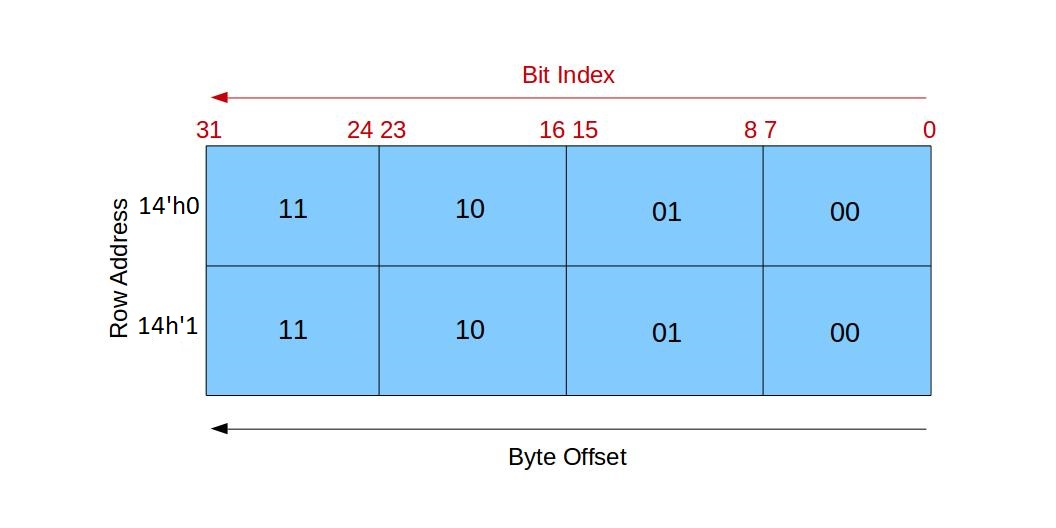
\includegraphics[width=0.8\textwidth]{figs/endianness_img.jpg}
    \caption{Block RAM organization.}
    \label{fig:endianness_img}
  \end{center}
\end{figure}

Figure \ref{fig:endianness_img} illustrates the 14-bit word addresses and the two bit byte offsets.
Observe that the RAM organization is \textbf{little-endian}, i.e. the most significant byte is at the most significant memory address (offset '11').

\subsubsection{Reading from RAMs}
Since the RAMs have 32-bit rows, you can only read data out of the RAM 32-bits at a time.
This is an issue when executing an \verb|lh| or \verb|lb| instruction, as there is no way to indicate which 8 or 16 of the 32 bits you want to read out.

Therefore, you will have to shift and mask the output of the RAM to select the appropriate portion of the 32-bits you read out.
For example, if you want to execute a \verb|lbu| on a byte address ending in \verb|2'b10|, you will only want bits \verb|[23:16]| of the 32 bits that you read out of the RAM (thus storing \verb|{24'b0, output[23:16]}| to a register).

\subsubsection{Writing to RAMs}
To take care of \verb|sb| and \verb|sh|, note that the \verb|we| input to the instruction and data memories is 4 bits wide.
These 4 bits are a byte mask telling the RAM which of the 4 bytes to actually write to.
If \verb|we|=\{4'b1111\}, then all 32 bits passed into the RAM would be written to the address given.

Here's an example of storing a single byte:
\begin{itemize}
  \item Write the byte \verb|8'ha4| to address \verb|32'h10000002| (byte offset = 2)
  \item Set \verb|we = {4'b0100}|
  \item Set \verb|din = {32'hxx_a4_xx_xx}| (\verb|x| means don't care)
\end{itemize}

\subsubsection{Unaligned Memory Accesses}
In the official RISC-V specification, unaligned loads and stores are supported.
However, in your project, you can ignore instructions that request an unaligned access.
Assume that the compiler will never generate unaligned accesses.


\subsection{Memory Architecture}
The standard RISC pipeline is usually depicted with separate instruction and data memories.
Although this is an intuitive representation, it does not let us modify the instruction memory to run new programs.
Your CPU, by the end of this checkpoint, will be able to receive compiled RISC-V binaries though the UART, store them into instruction memory, then jump to the downloaded program.
To facilitate this, we will adopt a modified memory architecture shown in Figure \ref{fig:mem_arch}.
Remember to assign their enebles properly in your logic.

\begin{figure}[hbt]
  \begin{center}
    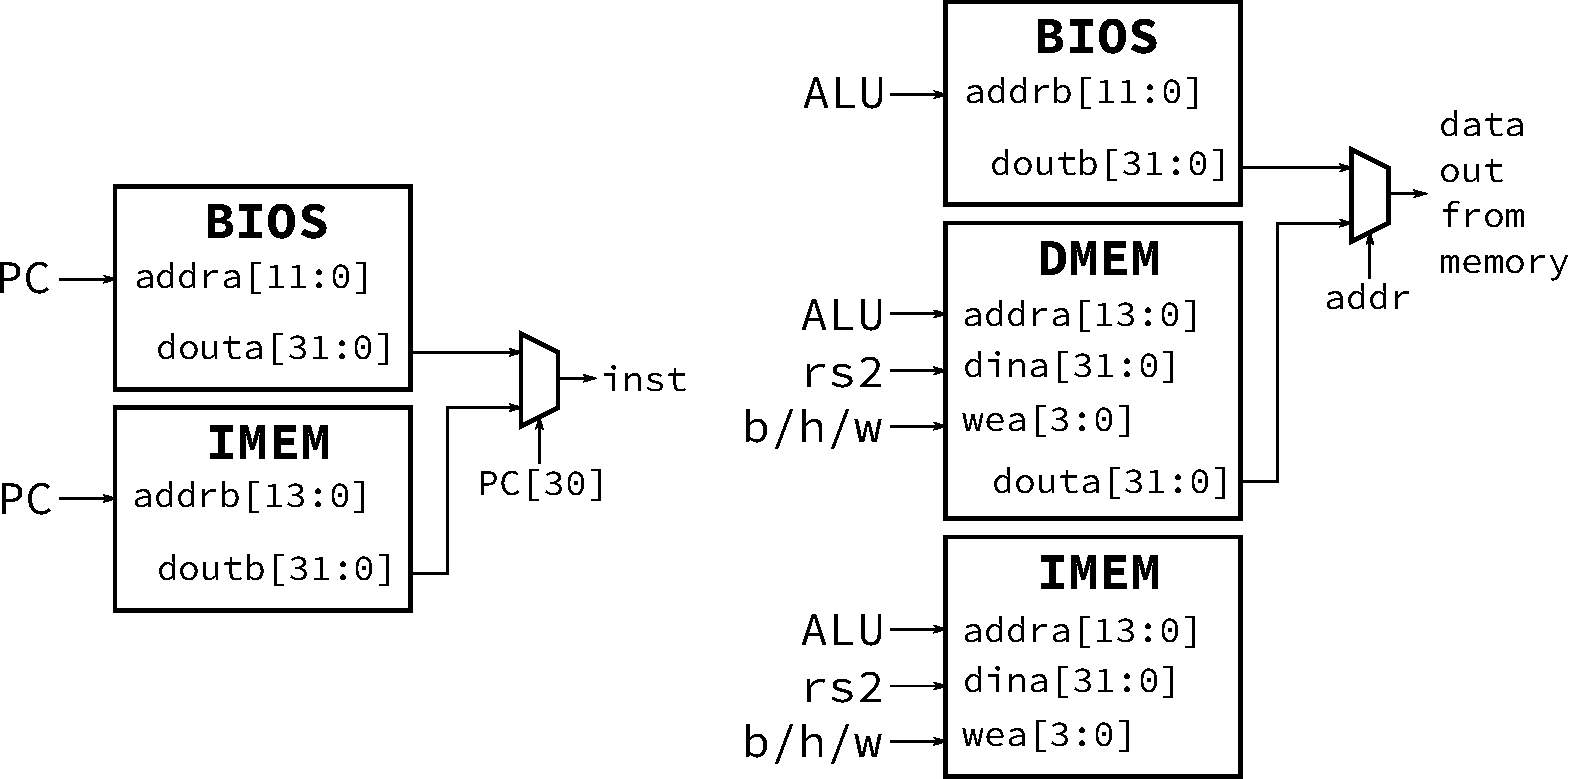
\includegraphics[width=0.8\textwidth]{figs/memory_arch.pdf}
    \caption{The Riscv151 memory architecture. There is only 1 IMEM and DMEM instance in your CPU but their ports are shown separately in this figure for clarity. The left half of the figure shows the instruction fetch logic and the right half shows the memory load/store logic.}
    \label{fig:mem_arch}
  \end{center}
\end{figure}

\subsubsection{Summary of Memory Access Patterns}
The memory architecture will consist of three RAMs (instruction, data, and BIOS).
The RAMs are memory resources (block RAMs) contained within the FPGA chip, and no external (off-chip DRAM) memory will be used for this project.

The processor will begin execution from the BIOS memory, which will be initialized with the BIOS program (in \verb|software/bios|).
The BIOS program should be able to read from the BIOS memory (to fetch static data and instructions), and read and write the instruction and data memories.
This allows the BIOS program to receive user programs over the UART from the host PC and load them into instruction memory.

You can then instruct the BIOS program to jump to an instruction memory address, which begins execution of the program that you loaded.
At any time, you can press the reset button (the right most button) on the board to return your processor to the BIOS program.

\subsubsection{Address Space Partitioning}
Your CPU will need to be able to access multiple sources for data as well as control the destination of store instructions.
In order to do this, we will partition the 32-bit address space into four regions: data memory read and writes, instruction memory writes, BIOS memory reads, and memory-mapped I/O.
This will be encoded in the top nibble (4 bits) of the memory address generated in load and store operations, as shown in Table \ref{fig:mem_space}.
In other words, the target memory/device of a load or store instruction is dependent on the address.
According to this partitioning, the reset signal should reset the PC to the value defined by the parameter \verb|RESET_PC| which is by default the base of BIOS memory (\verb|32'h40000000|).

The target memory/device is also dependent on the address type (PC or DATA).
For example the address beginning with \verb|4'h1| refers to the data memory when it is a data address, while it refers to the instruction memory when it is a program counter value.

\begin{table}[hbt]
  \begin{center}
    \caption{Memory Address Partitions}
    \label{fig:mem_space}
    \begin{tabular}{l l l l l}
      \bottomrule
      \textbf{Address[31:28]} & \textbf{Address Type} & \textbf{Device} & \textbf{Access} & \textbf{Notes} \\
      \midrule
      4'b0001 & PC   & Instruction Memory & Read-only  &\\
      4'b0100 & PC   & BIOS Memory        & Read-only  &\\
      4'b00x1 & Data & Data Memory        & Read/Write &\\
      4'b001x & Data & Instruction Memory & Write-Only & If PC[30] == 1'b1\\
      4'b0100 & Data & BIOS Memory        & Read-only  &\\
      4'b1000 & Data & I/O                & Read/Write &\\
      \bottomrule
    \end{tabular}
  \end{center}
\end{table}

Here are some examples.
When we are loading instructions, we are using a PC value as an address, and the instruction memory is read when it starts with \verb|4'h1|, while the BIOS memory is read when it starts with \verb|4'h4|.
On the other hand, when we are loading data by load instructions, the address type is Data, and the data memory is read when it starts with \verb|4'h1|, while the BIOS memory is read when it starts with \verb|4'h4|.

One tricky thing is that a store to an address beginning with \verb|4'h3| will write to both the instruction memory and the data memory, while storing to addresses beginning with \verb|4'h2| or \verb|4'h1| will write to either the instruction memory or the data memory, respectively.

\subsubsection{Memory Mapped I/O}
At this stage in the project the only way to interact with your CPU is through the UART.
The UART from Lab 5 accomplishes the low-level task of sending and receiving bits from the serial lines, but you will need a way for your CPU to send and receive bytes to and from the UART.
To accomplish this, we will use memory-mapped I/O, a technique in which registers of I/O devices are assigned memory addresses.
This enables load and store instructions to access the I/O devices as if they were memory.

To determine CPI (cycles per instruction) for a given program, the I/O memory map is also used to include instruction and cycle counters.

Table~\ref{fig:mem_map} shows the memory map for this stage of the project.

\begin{table}[hbt]
  \begin{center}
    \caption{I/O Memory Map}
    \label{fig:mem_map}
    \begin{adjustbox}{width=\columnwidth,center}
    \begin{tabular}{l l l l}
      \toprule
      \textbf{Address} & \textbf{Function} & \textbf{Access} & \textbf{Data Encoding}\\
      \midrule
      \verb|32'h80000000| & UART control & Read & \verb|{30'b0, uart_rx_data_out_valid, uart_tx_data_in_ready}| \\
      \verb|32'h80000004| & UART receiver data & Read & \verb|{24'b0, uart_rx_data_out}| \\
      \verb|32'h80000008| & UART transmitter data & Write & \verb|{24'b0, uart_tx_data_in}| \\
      \midrule
      \verb|32'h80000010| & Cycle counter & Read & Clock cycles elapsed \\
      \verb|32'h80000014| & Instruction counter & Read & Number of instructions executed \\
      \verb|32'h80000018| & Reset counters to 0 & Write & N/A \\
      \bottomrule
    \end{tabular}
    \end{adjustbox}
  \end{center}
\end{table}

You should treat I/O such as the UART just as you would treat the data memory.
The software checks the \verb|uart_rx_data_out_valid| and \verb|uart_tx_data_in_ready| signals by a load from \verb|32'h80000000|, and proceeds to a load from \verb|32'h80000004| or a store to \verb|32'h80000008| if the corresponding valid or ready signal is 1. Then your datapath will fetch \verb|uart_rx_data_out| or update \verb|uart_tx_data_in|, while asserting \verb|uart_rx_data_out_ready| or \verb|uart_tx_data_in_valid|, respectively.

The cycle counter should be incremented every cycle, and the instruction counter should be incremented for every instruction that is committed (you should not count bubbles injected into the pipeline or instructions run during a branch mispredict).
From these counts, the CPI of the processor can be determined for a given benchmark program.

\newpage

\section{\baseCPUTaskName: Implementation of RISC-V CPU}

This checkpoint requires a fully functioning three stage RISC-V CPU.
You need to demonstrate the BIOS functionality by loading the \verb|mmult| program over the UART,
and successfully jumping to and executing the program.
Additionally, please find the maximum achievable frequency
and report the critical path in your implementation.


\subsection{Testing}
\label{testing}
The design specified for this project is a complex system and debugging can be very difficult without tests that increase visibility of certain areas of the design.
In assigning partial credit at the end for incomplete projects, we will look at testing as an indicator of progress.
A reasonable order in which to complete your testing is as follows:

\begin{enumerate}
  \item Test your modules in isolation using testbenches that you write by yourself
  \item Test one instruction at a time with a hand-written assembly (\verb|sim/asm_tb.v|)
  \item Test that your CPU pipeline works with \verb|sim/cpu_tb.v|
  \item Test with the RISC-V ISA test suite (\verb|make isa-tests|)
  \item Test with other C programs in \verb|software/c_tests| (\verb|make c-tests|)
  \item Test the CPU's memory mapped I/O with \verb|uart_parse_tb.v| and \verb|echo_tb.v|
  \item Test the CPU's memory mapped I/O counters with \verb|mmio_counter_tb.v|
  \item Test the CPU's memory mapped I/O with the BIOS software program with \verb|bios_tb.v|
\end{enumerate}

Details are explained in Section \ref{sec:testing}.
You can run all tests other than \verb|mmio_counter_tb.v| by running
\begin{minted}{bash}
  ./script/run_all_sims.py
\end{minted}
in the \verb|hardware| directory.
The stdout/stderr will be dumped in \verb|hardware/test_results|.

Once you pass the BIOS testbench, you can implement and test your processor on the FPGA.


\subsection{Programming}
The build flow is identical to the labs.
Run \verb|make synth| in the \verb|hardware| directory to synthesize \verb|z1top|,
run \verb|make impl| to run place and route and bitstream generation,
and run \verb|make program| (or \verb|make remote|) to program the bitstream onto the FPGA.

Make sure you check the synthesis log in \verb|build/synth/synth.log|
for unexpected warnings before proceeding to place and route.

Execute the \verb|mmult| program on your FPGA, and verify its checksum.
Find the maximum clock frequency that can meet the timing constraints.
Look at the timing report and find the critical path in your implementation.
Instructions are explained in Section \ref{sec:programming}.


\subsection{How to Get Started}
It might seem overwhelming to implement all the functionality that your processor must support. The best way to implement your processor is in small increments, checking the correctness of your processor at each step along the way. Here is a guide that should help you plan out Checkpoint 2:

\begin{enumerate}
\item \textit{First steps.}
  Implement each of the components such as ALU.
  Unit test them.
\item \textit{Memory.}
  In the beginning, only use the instruction memory in the instruction fetch stage and only use the data memory in the memory stage.
  The BIOS memory is not used except in \verb|bios_tb.v|.
\item \textit{Connect stages and pipeline.}
  Connect your modules together and pipeline them.
  At this point, you should be able to run integration tests using assembly tests for most R and I type instructions.
\item \textit{Implement handling of control hazards.}
  Stall (insert bubbles) your pipeline to resolve control hazards if any, associated with JAL, JALR, and branch instructions.
  Don't worry about data hazards for now.
  Test that control instructions work properly with assembly tests.
\item \textit{Implement handling of data hazards.}
  Implement stalling or forwarding to resolve data hazards.
  Unless resolved by stalling, you have to forward to ALU inputs and memory data input.
  Test comprehensively; most of your bugs will come from incomplete or faulty handling of data hazards.
  At this point, your CPU should be able to pass the \verb|cpu_tb.v| test, \verb|isa-tests|, and \verb|c-tests|.
\item \textit{Integrate UART.}
  Add the UART to the memory stage, in parallel with the  instruction/data memories.
  Detect when an instruction is accessing the UART and route the data to the UART accordingly.
  Make sure that you are setting the UART ready/valid control signals properly
  as you are feeding or retrieving data from it.
  We have provided \verb|uart_parse_tb.v| and \verb|echo_tb.v| which performs a test of the UART.
\item \textit{Add instruction and cycle counters.}
  Add the memory mapped IO components, by first adding the cycle and instruction counters.
  These are just 2 32-bit registers that your CPU should update on every cycle and every instruction respectively.
  Verify it works using \verb|mmio_counter_tb.v|.
\item \textit{Add BIOS memory reads.}
  Add the BIOS memory to the memory stage to be able to load data from it.
  Write assembly tests that contain some static data stored in the BIOS memory
  and verify that you can read that data.
\item \textit{Add Inst memory writes and reads.}
  Add the instruction memory to the memory stage to be able to write data to it when executing inside the BIOS memory.
  Also add the BIOS memory to the instruction fetch stage to be able to read instructions from it.
  You may edit \verb|asm_tb.v| to test the functionality.
  Change the destination of \verb|$readmemh| to the BIOS memory,
  and update the initial program counter value, which is given to your CPU as a parameter.
  You may also have to change \verb|0x10000000| in \verb|asm.ld| to \verb|0x40000000|.
  Possible tests are first write instructions to the instruction memory,
  and then jump (using jalr) to instruction memory to see that the right instructions are executed.
  Test with \verb|bios_tb.v| to verify your CPU is fully functioning.
\item \textit{Run the BIOS.}
  If everything so far has gone well, program the FPGA.
  Verify that the BIOS performs as expected.
  As a precursor to this step, you might try to build a bitstream with the BIOS memory initialized with the echo program.
  To do so, change the \verb|STRINGIFY_BIOS| macro function in \verb|z1top.v| to \verb|x/../software/echo/echo.hex|.
\item \textit{Run matrix multiply.}
  Load the \verb|mmult| program with the \verb|hex_to_serial.py| script (located under \texttt{scripts}),
  and run \verb|mmult| on the FPGA. Verify that it returns the correct checksum.
  Check the CPI when running the \verb|mmult| program.
\end{enumerate}


\subsection{How to Succeed in This Checkpoint}
Start early and work on your design incrementally.
Keep the block diagram up to date as you write Verilog.
Unit test each component such as ALU, decoder, etc.
It is a good idea to separate those components into different modules (in different Verilog files), while instantiating them in your CPU module.
After testing your CPU pipeline with \verb|cpu_tb.v|, test with RISC-V ISA test suite and other C programs.
If your CPU is not working properly, you should go back to the assembly test to figure out the bug.
The final BIOS program is several 1000 lines of assembly and will be nearly impossible to debug by just looking at the waveform.

The most valuable asset for this checkpoint will not be your GSIs but will be your fellow peers who you can compare notes with and discuss design aspects with in detail.
However, do NOT under any circumstances share source code.

Once you're tired, go home and \textit{sleep}. When you come back you will know how to solve your problem.

\newpage

\section{Testing} \label{sec:testing}
\subsection{Unit Tests}
You should write unit tests for the isolated components of your CPU
such as the register file, decoder, and ALU in \verb|hardware/sim|.
The tests should contain assertions and check correct behavior
under several common and extreme conditions.

Run them just like you did in the labs.
For example, after you write \verb|sim/your_tb.v|, run \\
\verb|make sim/your_tb.fst| (iverilog) or \verb|make sim/your_tb.vpd| (VCS).
View the waveforms with \verb|gtkwave sim/your_tb.fst &| or \verb|dve -vpd sim/your_tb.vpd &|.

\subsection{Assembly Tests}
Once you connected the instruction memory in the instruction fetch stage and the data memory in the memory stage,
you should be able to run assembly tests using \verb|hardware/sim/asm_tb.v|.
Edit \verb|software/asm/start.s| by hand to add other tests you want.
It will be loaded into the instruction memory by the testbench,
where the \verb|RESET_PC| parameter is set to start the test in the IMEM instead of the BIOS.
Make sure you have used it in \verb|riscv_core/cpu.v|.

Initially, and if you change \verb|start.s|, you need to run \verb|make| in \verb|software|
before running simulation.

The \verb|start.s| contains the following instructions.
\begin{minted}{asm}
  # Test ADD
  li x10, 100         # Load argument 1 (rs1)
  li x11, 200         # Load argument 2 (rs2)
  add x1, x10, x11    # Execute the instruction being tested
  li x20, 1           # Set the flag register for the testbench
  # Now we check that x1 contains 300 in the testbench
\end{minted}
The \verb|asm_tb| toggles the clock one cycle at time and waits for register \verb|x20|
to be written with a particular value (in the above example: 1).
Once \verb|x20| contains 1, the testbench inspects the value in \verb|x1|
and checks if it is 300, which indicates your processor correctly executed the add instruction.

If the testbench times out it means \verb|x20| never became 1,
so the processor got stuck somewhere or \verb|x20| was written with another value.

You should add your own tests to verify that your processor can execute
different instructions correctly.
Modify and compile \verb|start.s| with your tests, add your checks to \verb|asm_tb.v|,
and then rerun the RTL simulation.

\subsection{CPU Test}
Once you are confident that your processor is working,
you will want to perform a comprehensive test.
The provided \verb|sim/cpu_tb.v| tests all the RV32I instructions.

To pass this testbench, you should have a working CPU implementation that can decode and execute
all the instructions in the spec, including the CSR instructions.
Several basic hazard cases are also tested.

Unlike other testbenches, this testbench does not work with any software code,
but rather it manually initializes the instructions and data in the memory blocks
as well as the register file content for each test.
The testbench does not cover reading from BIOS memory nor memory mapped IO.

\subsection{RISC-V ISA Tests}
These are tests developed in the RISC-V community.
To run the tests, run \verb|make isa-tests| or \verb|make sim/isa/lw.fst| for a specific test.

The simulation log details which tests passed and failed and the number of clock cycles elapsed.
If you're failing a test, debug using the generated assembly dump in
\verb|software/riscv-isa-tests|.

The assembly dump files are extremely helpful in debugging at this stage.
If you look into a particular dump file of a test (e.g., \verb|add.dump|),
it contains several subtests in series.
The CSR output from the simulation indicates which subtest is failing
to help you narrow down where the problem is, and you can start debugging from there.

\subsection{C Tests}
Next, you will test your processor with some small RISC-V C programs.
The C tests are in \verb|software/c_tests|.
You should go into each folder, understand what the program is trying to do.
The available tests are \verb|strcmp|, \verb|vecadd|, \verb|fib|, \verb|sum|,
\verb|replace|, and \verb|cachetest|.

To run the test, run \verb|make c-tests| or \verb|make sim/c_tests/fib.fst| for a specific program.
These tests could help reveal more hazard bugs in your implementation.
\verb|strcmp| is particularly important since it is frequently used in the BIOS program.

The tests use CSR instruction to indicate if they are passed
(e.g., write 1 to the CSR register if passed).
Following that practice, you can also write your custom C programs to further test your CPU.

As an additional tip for debugging, try changing the compiler optimization flag in the Makefile
of each software test (e.g., \verb|-O2| to \verb|-O1| or \verb|-O0|),
and see if your processor still passes the test.
Different compiler settings generate different sequences of assembly instructions,
and some might expose subtle hazard bugs yet to be covered by your implementation.

\subsection{UART and Echo Tests}
You should have your UART modules integrated with the CPU before running these tests.
These tests verify if your CPU is able to: check the UART status,
read a character from UART Receiver, and write a character to UART Transmitter.

Take a look at the software code \verb|software/echo/echo.c| to see what it does.
The testbench sends several characters over the serial rx line and sees if they are returned correctly.
The \verb|software/uart_parse/uart_parse.c| emulates the first few instructions of BIOS program.
The testbench checks if it sends and receives the correct sequence.

\subsection{MMIO Counter Test}
This test executes NOPs and a for loop with 10 iterations,
and prints out the values of counters for each.

Remember that we don't include NOPs in the instruction count,
and that only the completed instructions are counted
(the instructions that have passed the last stage of your pipeline).
The expected values for the instruction counts are around
2 (reset counters and load cycle count)
and 23 (loop initialization and 2 * 10 for loop iterations besides the previous two).

\subsection{BIOS Test}
We have provided a BIOS program in \verb|software/bios| that allows you to interact
with your CPU and download other programs over UART.
The BIOS program is an infinite loop that reads from the UART,
checks if the input string matches a known control sequence,
and then performs an associated action.
For detailed information on the BIOS, see Section \ref{sec:bios}.

The BIOS testbench \verb|sim/bios_tb.v| emulates the interaction between
the host and your CPU via the serial lines orchestrated by the BIOS program.
It tests four basic functions of the BIOS program:
\begin{itemize}
\item sending an invalid command
\item storing to an address (in IMEM or DMEM)
\item loading from an address (in IMEM or DMEM)
\item jumping to an address (from BIOSMEM to IMEM)
\end{itemize}


\newpage

\section{Programming} \label{sec:programming}
\subsection{Manual Tests}
After programming, open screen to access the serial port:
\begin{minted}{bash}
  screen $SERIALTTY 115200
\end{minted}
Press the reset button (the right most button) to make the CPU PC go to the start of BIOS memory.

If all goes well, you should see a \verb|151 >| prompt after pressing return.
The following commands are available:
\begin{itemize}
\item \verb|jal <address>|: Jump to address (hex)
\item \verb|[sw, sb, sh] <data> <address>|: Store data (hex) to address (hex).
\item \verb|[lw, lbu, lhu] <address>|: Prints the data at the address (hex).
\end{itemize}
If your backspace doesn't work, try \verb|Ctrl-Backspace|

As an example, running \verb|sw cafef00d 10000000| should write to the data memory
and running \verb|lw 10000000| should print the output \verb|10000000: cafef00d|.
Please also pay attention that writes to the instruction memory .
You may try \verb|sw ffffffff 20000000| that writes to the data memory,
where \verb|lw 10000000| still should yield \verb|cafef00d|.

Once you're done, make sure that you close screen using \verb|Ctrl-a| \verb|Shift-k|,
or other students won't be able to use the serial port!
If you can't access the serial port you can run \verb|killscreen| to kill all screen sessions.

\subsection{Loading Software Programs}
In addition to the command interface,
the BIOS allows you to load programs to the CPU.
With {\bf screen closed}, run:
\begin{minted}{bash}
  ./scripts/hex_to_serial.py <hex_file> <address>
\end{minted}
This script stores the hex file at the specified hex address.

In order to run the software program,
you need to write into both the data and instruction memories,
remember to set the top nibble of the address to \verb|0x3| as follows:
\begin{minted}{bash}
  ./scripts/hex_to_serial.py ../software/echo/echo.hex 30000000
\end{minted}
Then, you should jump to the loaded instructions in your screen session by \verb|jal 10000000|.
In this case, as you loaded the echo program, you should see the characters you typed
sent back and printed on your screen.

After you make sure that your FPGA are executing the loaded program correctly,
reset your FPGA and try the mmult program in \verb|../softwar/mmult/mmult.hex|.

This program computes $S=AB$, where $A$ and $B$ are $64 \times 64$ matrices.
The program will print a checksum and the counters discussed in Memory Mapped IO.
The correct checksum is \verb|0001f800|.
If nothing printed out, there is likely a problem in your CPU with one of the instructions that is used by the BIOS but not mmult.

The program will also output the values of your instruction and cycle counters (in hex).
These can be used to calculate the CPI for this program.

\subsection{Target Clock Frequency}
By default, the CPU clock frequency is set at 50~MHz.
It should be easy to meet timing at 50~MHz.
Please try higher frequencies by decreasing the \verb|CPU_CLOCK_PERIOD| parameter
(starting at 20, with a step size of 1) in \verb|hardware/src/z1top.v|.
The unit of the clock period is ns,
e.g. \verb|CPU_CLOCK_PERIOD = 10| means 10~ns clock period and 100~MHz frequency.
Placement and route (\verb|make impl|) will take more time if you use a higher frequency.

If you found the following line in \verb|build/impl/impl.log|
(also displayed when \verb|make impl|), routing failed:
\begin{minted}[breaklines]{bash}
  CRITICAL WARNING: [Timing 38-282] The design failed to meet the timing requirements. Please see the timing summary report for details on the timing violations.
\end{minted}
The detailed report can be found at \verb|build/impl/post_route_timing_summary.rpt|.
You may copy that file to the \verb|doc| directory for your record.
The section \verb|Max Delay Paths| shows the critical path in your design.
The slack is negative if routing failed, showing how much delay we need to reduce in the path
to meet the timing constraints.
The signals names may have been changed during optimization.
You may refer to \verb|build/impl/post_route.v| or \verb|build/synth/post_synth.v|
to figure out what they correspond to in your source code.


\newpage

\section{Optimization}
\subsection{Overview}
Project requirements and grading will be different this semester than in recent semesters.
We would like to be as fair as possible and to give you an experience that closely matches what you will find in industry.
Therefore we will assign your project grade using a {\em figure of merit (FOM)} computed based on your design.
The FOM in this case will be a combination of your processor's maximum clock frequency ($F_{max}$), average cycles per instruction (CPI), and cost:

$$ FOM = \frac{F_{max}}{CPI \cdot cost}$$


$F_{max}$ is the maximum clock frequency at which your processor correctly passes our test benchmarks.
CPI is the average cycle per instruction for your processor running our benchmarks, as described below.
Cost will be based on which and how many FPGA elements your design includes, as detailed in the post place synthesis report.
It will be computed using a script that processes your report and forms a weighted sum of all the elements in your design.
The weights correspond to the relative chip area that each element occupies.  {\em We will not, however, include the cost of FPGA block RAM memory elements.}

We include {\em cost} in the FOM because we want to encourage simpler designs.
Experience shows that debugging times increases very quickly with design complexity, and in the past many students
have had trouble debugging complex designs by the end of the semester.
You will have a much better experience and learn more by keeping your design simple.
On the other hand, we would like you to explore options for improving performance.
But while doing so you should be mindful of whether or not extra complexity to improve performance is worth the extra cost.
Therefore if you are tempted to add complexity, make sure that it will actually improves the FOM.

The lab grading break down will be as follows:
\begin{description}
\item[50\%] Correctly functioning 3-stage (at least) processor, without regard for performance and cost.
\item[35\%] FOM optimizations.
\item[5\%] Checkpoints.
\item[10\%] Final report.
\end{description}

Once you have a functionally correct processor, the next steps will be to modify it to achieve a higher FOM and thus achieve a higher grade.
We will give you suggestions on how to maximize the FOM (and therefore your grade),
but it will be up to you to make good decisions as to how to optimize your design.

For purposes of computing the FOM, we will rely on two counters that you are required to implement as described in the project specification document.
One counts cycles and the other counts instructions.
%The RISC-V BIOS includes a command (``run'') for running a program.
Our benchmarks automatically clear the counters and reports the counts after the run.  In addition to using our benchmark programs you are welcome to write your own.
We will provide a script that takes as input the two counter values, your $F_{max}$, and a report (.rpt) file, and outputs the CPI and the FOM values.
For final checkoff we will use the $F_{max}$ value from running your processor on the FPGA board and will use the ``post\_place\_utilization.rpt'' file to determine the cost.
However, since place and route might take significant time as your design grows in complexity, to speed up your design space exploration, you might want
to use the ``post\_synth\_utilization.rpt'' file for costs, estimate $F_{max}$ based on your synthesis target and available slack from the timing report, and use simulation to get the cycle and instruction counts.  However, becasuse the simulator is significantly slower than running on the actual FPGA, this approach will only work for small benchmark programs.


It should go without saying that to improve the FOM, you will need to increase $F_{max}$, decrease $CPI$, decrease cost, or some combination of these.
You should be able to improve $F_{max}$ without substantially changing the microarchitecture of your design
by shortening the critical path.
Of course, after you improve one path, you might then want to optimize the next longest.
Improving a path could come down to how you write the Verilog, or you might need to rearrange the logic.
Also, obviously, increasing the number of pipeline stages might also shorten the critical path, but such a change could have an adverse effect on CPI and cost; so proceed with caution.
In this design, a small Dcache and/or Icache might also help improve $F_{max}$, if you can find a way to build a cache that is substantially faster than block RAM.
To improve CPI, you might consider using branch prediction.
Also, you might even want to consider mechanisms that would bring CPI below 1 --- however, these mechanisms can get tricky to design.
If you have other ideas and are unsure if it will help, feel free to talk with us and get our feedback before investing time in an idea that may or may not work out.

For a 3-stage unoptimized design, we expect typical values around: $F_{max}$ = 60~MHz, CPI = 1.5, and cost = 1.5~M, and therefore a FOM of around 25.

At a later date we will post approximate FOM grade targets (what FOM values correspond to project point assignments).
Also, we will try to find a way to occasionally anonymously post updates on FOM values that other groups have achieved.


\subsection{Scripts}
Several scripts are provided to calculate the FOM of your design.
After compiling the programs (\verb|make| in the \verb|software| directory),
you can simply run
\begin{minted}{bash}
  ./script/fom.py
\end{minted}
in the \verb|hardware| directory.
It returns the estimated FOM based on CPIs for small benchmarks.
Since we have multiple benchmark programs (we will add more later),
the CPI is calculated as a geometric mean of all benchmarks.

To get the actual FOM using the real CPI, use \verb|-r| option.
It calls \verb|run_fpga.py| for all benchmarks to obtain the real CPI.
Make sure you program the FPGA and close your screen before running the script.

The cost is calculated based on one of the following:
\begin{itemize}
\item \verb|./build/synth/post_synth_utilization.rpt|
\item \verb|./build/impl/post_place_utilization.rpt|
\end{itemize}
By default, the \verb|fom.py| script compares the last modification time and uses the newer one.
You can force it to use \verb|./build/synth/post_synth_utilization.rpt| with \verb|-s| option,
or the other one with \verb|-i| option.
Use \verb|-u| option to specify the report in other location.
Note that for the final grade, we will use \verb|./build/impl/post_place_utilization.rpt|.

The maximum frequency is automatically read from timing summary reports:
\begin{itemize}
\item \verb|./build/synth/post_synth_timing_summary.rpt|
\item \verb|./build/impl/post_rote_timing_summary.rpt|
\end{itemize}
\verb|clk_out1_design_1_clk_wiz_0_1| in the report is the clock signal driving your CPU.
By default, it uses the one in the same directory as the selected resorce utilization report.
You can manually specify it with \verb|-t| option.
Again, we will use \verb|./build/impl/post_rote_timing_summary.rpt| for the final grade.
Do not forget to adjust \verb|CPU_CLOCK_PERIOD| in \verb|z1top.v| after you modified your datapath.
The detailed instructions are in Sec. \ref{sec:target_clock_frequency}.

You can manually override each of cost, $F_{max}$, and CPI with \verb|-c|, \verb|-f|, and \verb|-p| option, respectively.

The following boxes show the log of \verb|fom.py| on unoptimized 2-stage pipeline for your reference.
After some exploration, the maximum frequency for this design turned out to be 62.5~MHz (\verb|CPU_CLOCK_PERIOD=15|).
The estimated FOM was 30.54 as shown below.
\usemintedstyle{bw}
\begin{minted}[breaklines, frame=single]{bash}
$ ./scripts/fom.py
Using build/impl/post_place_utilization.rpt (last modified: Wed Apr  5 03:06:32 2023)
Using build/impl/post_route_timing_summary.rpt (last modified: Wed Apr  5 03:08:05 2023)
Running simulation...
Result: 000000e0
Cycle Count: 00005483
Instruction Count: 00004476
[     27974 sim. cycles] mmult PASSED!
Result: 0000004f
Cycle Count: 00007d03
Instruction Count: 00005bf3
[     37929 sim. cycles] bdd PASSED!
...simulation complete
Cycle Counts: [21635, 32003]
Instruction Counts: [17526, 23539]
CPIs: [1.23, 1.36]
CPI (geomean): 1.30

Fmax: 62.5
CPI: 1.30
Cost: 1579727

FOM (estimate): 30.54
\end{minted}

For the actual FOM, we have to run the benchmarks on the FPGA with \verb|-r| option.
Here, as an example, we manually gave cost and $F_{max}$.
\usemintedstyle{bw}
\begin{minted}[breaklines, frame=single]{bash}
$ ./scripts/fom.py -r -f 62.5 -c 1579727
Running on FPGA...
Sending command: file 30000000 6100
Sent 6100/6100 bytes
Done
Sending command: run
Result: 000017a4
Cycle Count: 0057e4d8
Instruction Count: 003d2ef4
Done
Sending command: file 30000000 2368
Sent 2368/2368 bytes
Done
Sending command: run
Result: 0001f800
Cycle Count: 00f50332
Instruction Count: 00c4c2ed
Done
...FPGA run complete
Cycle Counts: [5760216, 16057138]
Instruction Counts: [4009716, 12894957]
CPIs: [1.44, 1.25]
CPI (geomean): 1.34

Fmax: 62.5
CPI: 1.34
Cost: 1579727

FOM: 29.58
\end{minted}

As you can see, the real CPIs are different from what we got in simulation,
since benchmark sizes are different.
That is, you should compare an estimated FOM with another estimated FOM,
and an actual FOM with another actual FOM, not in a mixed manner.


\newpage



\begin{appendices}
\section{BIOS}
\label{sec:bios}
This section was written by Vincent Lee, Ian Juch, and Albert Magyar.
Updated by Yukio Miyasaka.

\subsection{Background}
For the first checkpoint we have provided you a BIOS written in C that your processor is
instantiated with. BIOS stands for Basic Input/Output System and forms the bare bones of the
CPU system on initial boot up. The primary function of the BIOS is to locate, and initialize the
system and peripheral devices essential to the PC operation such as memories, hard drives, and
the CPU cores.

Once these systems are online, the BIOS locates a boot loader that initializes the operating
system loading process and passes control to it. For our project, we do not have to worry about
loading the BIOS since the FPGA eliminates that problem for us. Furthermore, we will not deal
too much with boot loaders, peripheral initialization, and device drivers as that is beyond the
scope of this class. The BIOS for our project will simply allow you to get a taste of how the
software and hardware layers come together.

The reason why we instantiate the memory with the BIOS is to avoid the problem of
bootstrapping the memory which is required on most computer systems today. Throughout the
next few checkpoints we will be adding new memory mapped hardware that our BIOS will
interface with. This document is intended to explain the BIOS for checkpoint 1 and how it
interfaces with the hardware. In addition, this document will provide you pointers if you wish to
modify the BIOS at any point in the project.

\subsection{Loading the BIOS}
For the first checkpoint, the BIOS is loaded into the Instruction memory when you first build it.
As shown in the Checkpoint 1 specification, this is made possible by instantiating your
instruction memory to the BIOS file by building the block RAM with the \verb|bios.hex| file. If you
want to instantiate a modified BIOS you will have to change this .hex file in your block RAM
directory and rebuild your design and the memory.

To do this, simply cd to the \verb|software/bios| directory and make the .hex file by running
“make”. This should generate the .hex file using the compiler tailored to our ISA. The
block RAM will be instantiated with the contents of the .hex file.
When you get your design to synthesize and program the board, open up screen using the
same command from Lab 5:

\verb|screen $SERIALTTY 115200|

or

\verb|screen /dev/ttyUSB0 115200|

Once you are in \verb|screen|, if you CPU design is working correctly you should be able to hit Enter
and a carrot prompt \verb|'>'| will show up on the screen. If this doesn’t work, try hitting the reset
button on the FPGA. If you can’t get the BIOS
carrot to come up, then your design is not working and you will have to fix it.

\subsection{Loading Your Own Programs}
The BIOS that we provide you is written so that you can actually load your own programs for
testing purposes and benchmarking. Once you instantiate your BIOS block RAM with the
\verb|bios.hex| file and synthesize your design, you can transfer your own program files over the
serial line.

To load you own programs into the memory, you need to first have the .hex file for the program
compiled. You can do this by copying the software directory of one of our C programs folders in
\verb|software| directory and editing the files. You can write your own RISC-V program by writing
test code to the .s file or write your own c code by modifying the .c file.
Once you have the .hex file for your program, impact your board with your design and run:

\verb|./script/hex_to_serial.py <file name>|

The \verb|<file name>| field corresponds to the .hex file that you are to uploading to the instruction
memory.

Once you have uploaded the file, you can fire up screen and run the command:

\verb|run|

Note that the instruction memory size is limited in address size so large programs may fail to load.


\subsection{The BIOS Program}
The BIOS itself is a fairly simple program and composes of a glorified infinite loop that waits for
user input. If you open the \verb|bios.c| file, you will see that the main method composes of a
large for loop that prints a prompt and gets user input by calling the \verb|read_token| method.
If at any time your program execution or BIOS hangs or behaves unexpected, you can hit the
reset button, the rightmost button on your board, to reset the program execution to the main method.
The \verb|read_token| method continuously polls the UART for user input from the keyboard until it
sees the character specified by ds. In the case of the BIOS, the termination character
\verb|read_token| is called with is the 0xd character which corresponds to Enter.
The \verb|read_token| method will then return the values that it received from the user.

\begin{figure}[H]
  \centering
  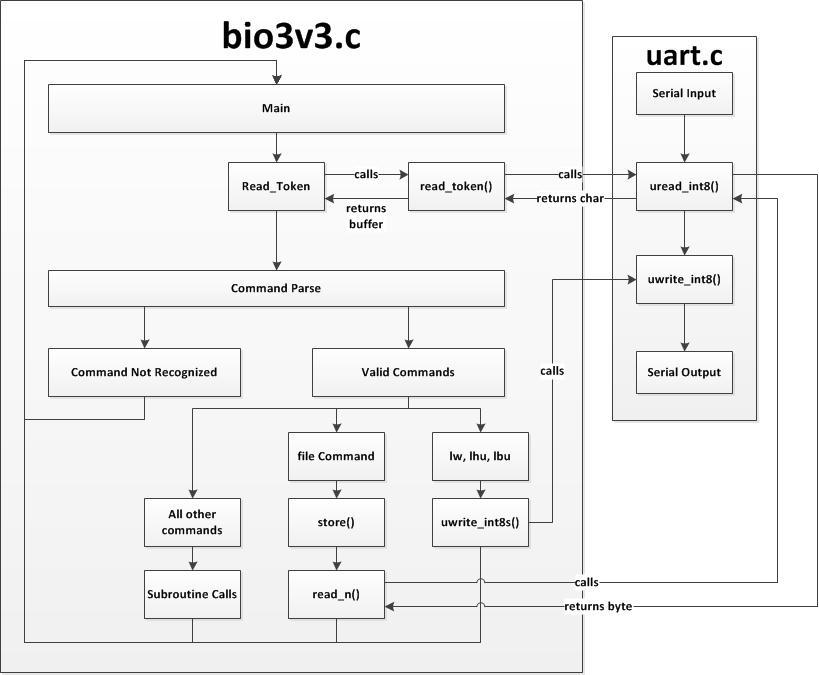
\includegraphics[width=0.7\textwidth]{figs/bios_flow.png}
  \caption{BIOS Execution Flow}
\end{figure}

The buffer returned from the \verb|read_token| method with the user input is then parsed by
comparing the returned buffer against commands that the BIOS recognizes. If the BIOS parses a
command successfully it will execute the appropriate subroutine or commands. Otherwise it
will tell you that the command you input is not recognized.
If you want to add commands to the BIOS at any time in the project, you will have to add to the
comparisons that follow after the \verb|read_token| subroutine in the BIOS.

\subsection{The UART}
You will notice that some of the BIOS execution calls will call subroutines in the uart.c file
which takes care of the transmission and reception of byte over the serial line.
The uart.c file contains three subroutines. The first subroutine, \verb|uwrite_int8| executes a
UART transmission for a single byte by writing to the output data register. The second
subroutine \verb|uwrite_int8s| allows you to process an array of type \verb|int8_t| or chars and send
them over the serial line. The third routine \verb|uread_int8| polls the UART for valid data and
reads a byte from the serial line.

In essence, these three routines are operating the UART on your design from a software view
using the memory mapped I/O. Therefore, in order for the software to operate the memory
map correctly, the \verb|uart.c| module must store and load from the correct addresses as defined
by out memory map. You will find the necessary memory map addresses in the uart.h file that
conforms to the design specification.

\subsection{Command List}
The following commands are built into the BIOS that we provide for you. All values are
interpreted in hexadecimal and do not require any radix prefix (ex. ``0x''). Note that there is not
backspace command.

\verb|jal <hexadecimal address>| - Moves program execution to the specified address

\verb|lw <hexadecimal address>| - Displays word at specified address to screen

\verb|lhu <hexadecimal address>| - Displays half at specified address to screen

\verb|lbu <hexadecimal address>| - Displays byte at specified address to screen

\verb|sw <value> <hexadecimal address>| - Stores specified word to address in memory

\verb|sh <value> <hexadecimal address>| - Stores specified half to address in memory

\verb|sb <value> <hexadecimal address>| - Stores specified byte to address in memory

\verb|run| - Alias of \verb|jal 10000000|

There is another command \verb|file| in the main() method that is used only when you execute \\
\verb|hex_to_serial.py|. When you execute \verb|hex_to_serial.py|, your workstation will initiate a byte
transfer by calling this command in the BIOS. Therefore, don’t mess with this command too
much as it is one of the more critical components of your BIOS.

\subsection{Adding Your Own Features}
Feel free to modify the BIOS code if you want to add your own features during the project for
fun or to make your life easier. If you do choose to modify the BIOS, make sure to preserve
essential functionality such as the I/O and the ability to store programs. In order to add
features, you can either add to the code in the \verb|bios.c| file or create your own c source and
header files. Note that you do not have access to standard c libraries so you will have to add
them yourself if you need additional library functionality.

\newpage

\end{appendices}

\end{document}
